\documentclass[12pt,a4paper]{article}
\usepackage[utf8]{inputenc}
\usepackage[portuguese]{babel}
\usepackage[T1]{fontenc}
\usepackage{amsmath}
\usepackage{amsfonts}
\usepackage{amssymb}
\usepackage{graphicx}
\usepackage[left=2cm,right=2cm,top=2cm,bottom=2cm]{geometry}
\author{Gabriel de Albuquerque Mendes,\\
 João Pedro Abreu de Souza e \\
 Maqueise de Medeiros Pinheiro}
\title{Resolvendo o 8-Puzzle com algoritmos de busca em Prolog}
\date{19 de Novembro de 2019}

\begin{document}
\maketitle
O \textit{8-Puzzle} (ou quebra-cabeça de 8 peças) é um quebra-cabeça composto por uma caixa oca com 8 peças deslizantes dentro, todas numeradas de 1 à 8. O objetivo do jogo é arrumar as peças de forma que os números fiquem em ordem crescente e um espaço no final.

Nosso trabalho visa resolver o 8-Puzzle utilizando algoritmos de busca implementados em Prolog.
\\

O quebra-cabeça foi implementado em formato de lista, sendo as peças numeradas representadas por seus próprios algarismos e o espaço como \textit{"blank"}. Dessa forma, um configuração
\begin{center}
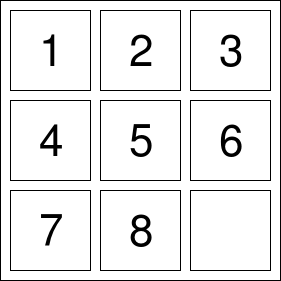
\includegraphics[scale=0.5]{8puzzle.png} 
\end{center} 
se tornaria $$[1,2,3,4,5,6,7,8,blank].$$
\\

Inicialmente, foi feito um algoritmo utilizando \textbf{busca em profundidade}. Essa abordagem não se mostrou eficiente, já que movimentava o jogo de acordo com a ordem na qual foi estabelecido os espaços vizinhos, fazendo assim uma série de movimentos desnecessários até a eventual obtenção do resultado.

Quando por exemplo a entrada do algoritmo é $[1,2,3,4,5,6,7,8,blank]$, ou seja, o resultado, ele retorna a mesma lista sem problemas. Mas quando é uma entrada cujo a solução também deveria ser simples como $[1,2,3,4,5,6,7,blank,8]$ que tem apenas uma peça fora do lugar, o algoritmo retorna tantos movimentos até a solução que não é possivel ver todas pelo prolog. E ainda com a lista de entrada $[1,8,2,blank,4,3,7,6,5]$, a busca nem chega a retornar algo.
\\

Em seguida, foi construido um algoritmo usando \textbf{busca em largura}. Esse método de busca se mostrou mais eficaz que o anterior, com caminhos mais diretos até o resultado. Entretanto, em alguns casos de teste, o consumo de memória foi excessivo devido a sua necessidade de expandir os caminhos antes de prosseguir.

Quando a entrada é $[1,2,3,4,5,6,7,8,blank]$ também retorna sem problemas. No caso da entrada $[1,2,3,4,5,6,7,blank,8]$ faz apenas o único movimento necessário e na entrada $[1,8,2,blank,4,3,7,6,5]$ acha a solução em apenas 10 movimentos.
\\

A \textbf{busca ótima (busca A*)} teve o melhor resultado. Além de eficiente se mostrou mais rápida que as demais. Foi feito um algoritmo usando a \textit{Distância de Manhattan}\footnote{Dado dois vetores $X=(X_1,X_2,...,X_p)$ e $Y=(Y_1,Y_2,...,Y_p)$, a \textbf{Distância de Manhattan} é definida como o somatório dos módulos das diferenças. $$d(X,Y)= \sum_{i=1}^{p} \mid X_i - Y_i \mid$$} como estimativa de custo e outro utilizando a \textit{Distância de Hamming}\footnote{A \textbf{Distância de Hamming} entre duas strings de mesmo comprimento é o número de posições nas quais elas diferem entre si.}.

Utilizando a Distância de Manhattan, os dois primeiros exemplos de entrada,  $[1,2,3,4,5,6,7,8,blank]$ e $[1,2,3,4,5,6,7,blank,8]$, se comportam da mesma maneira que a busca em largura.

Utilizando a Distância de Hamming, todos os retornos foram semelhantes ao da busca em largura.

\end{document}